\chapter{Triển khai ứng dụng}
\label{Chapter4}

\emph{Chương này sẽ trình bày, mô tả chi tiết về quá trình triển khai ứng dụng, kết quả phân tích bài toán chỉ đường, đưa ra các yêu cầu cụ thể cho bài toán. Đồng thời chương này cũng trình bày bản thế kế kiến trúc hệ thống và các thiết kế chi tiết khác.}

\section{Phân tích, đặc tả yêu cầu}

\subsection{Mô tả chung}
Sản phẩm là một ứng dụng cho phép người dùng ghi âm giọng nói hoặc nhập văn bản, sau đó tự phân tích giọng nói về văn bản để xác định yêu cầu và hướng dẫn đường đi. Sản phẩm cung cấp giao diện để người dùng có thể ghi âm và nhập văn bản trên ứng dụng di động một cách dễ dàng.
Mục đích của ứng dụng chatbot chỉ đường là cung cấp một giao diện thân thiện, người dùng có thể dễ dàng hỏi những câu hỏi liên quan đến đường đi bằng văn bản hoặc giọng nói và nhận câu trả lời ngay lập tức.
\subsection{Yêu cầu chức năng}

Yêu cầu chức năng chỉ đường từ một điểm đến một điểm bằng văn bản:
\begin{itemize}
    \item[--] Dữ liệu vào: Yêu cầu của người dùng dưới dạng văn bản
    \item[--] Xử lý: Thiết bị nhận văn bản để biết yêu cầu của người dùng. Nếu yêu cầu được hỗ trợ, hệ thống xử lý yêu cầu đó và phản hồi bằng giọng nói và văn bản cho người dùng. Nếu yêu cầu không được hỗ trợ, thiết bị phản hồi yêu cầu không được hỗ trợ bằng giọng nói và văn bản.
    \item[--] Kết quả: Phản hồi bằng văn bản hiển thị lên màn hình ứng dụng và giọng nói của thiết bị.
\end{itemize}
Yêu cầu chức năng chỉ đường từ một điểm đến một điểm bằng âm thanh (audio):
\begin{itemize}
    \item[--] Dữ liệu vào: Yêu cầu của người dùng dưới dạng audio
    \item[--] Xử lý: Thiết bị biến giọng nói vào thành văn bản để biết yêu cầu của người dùng. Nếu yêu cầu được hỗ trợ, hệ thống xử lý yêu cầu đó và phản hồi bằng giọng nói và văn bản cho người dùng. Nếu yêu cầu không được hỗ trợ, hệ thống phản hồi yêu cầu không được hỗ trợ bằng giọng nói và văn bản.
    \item[--] Kết quả: Phản hồi bằng văn bản hiển thị lên màn hình ứng dụng và giọng nói của thiết bị.
\end{itemize}



\subsection{Yêu cầu giao diện phần mềm}

Yêu cầu giao diện cho chức năng cho ứng dụng chỉ đường : Giao diện đơn giản, dễ sử dụng

Yêu cầu giao diện cho chức năng Chat chỉ đường bằng văn bản:
\begin{itemize}
    \item[--] Giao diện đơn giản, dễ sử dụng
    \item[--] Câu lệnh ngắn gọn, dễ ghi
    \item[--] Phản hồi ngắn gọn dễ nghe, dễ đọc
    \item[--] Phản hồi mọi câu lệnh dù câu lệnh đó không được hỗ trợ
\end{itemize}

Yêu cầu giao diện cho chức năng Chat chỉ đường bằng giọng nói:
\begin{itemize}
    \item[--] Giao diện đơn giản, dễ sử dụng
    \item[--] Câu lệnh ngắn gọn, dễ đọc
    \item[--] Phản hồi ngắn gọn, dễ nghe, dễ đọc
    \item[--] Phản hồi mọi câu lệnh dù câu lệnh đó không được hỗ trợ
    \item[--] Phải có giao diện ghi âm để phản hồi trực quan
\end{itemize}

\subsection{Yêu cầu hiệu suất}
\begin{itemize}
    \item[--] Thiết bị phải hoạt động được liên tục trong thời gian dài, từ 12 đến 24 giờ
    \item[--] Kết quả chỉ đường phải đạt độ chính xác tối thiểu 80\%
    \item[--] Tốc độ phản hồi phải nhỏ hơn 5 giây
    \item[--] Đảm bảo sự kết nối của nhiều ứng dụng cùng một thời điểm lên hệ thống
\end{itemize}

\subsection{Ràng buộc thiết kế}
\begin{itemize}
    \item[--] Sản phẩm phải được thiết kế bằng tiếng Việt, bao gồm giao diện người dùng, các phản hồi bằng giọng nói và văn bản
    \item[--] Sản phẩm ứng dụng cần đảm bảo tính thẩm mỹ
\end{itemize}

\subsection{Ràng buộc thuộc tính}
\begin{itemize}
    \item[--] Cơ sở dữ liệu phải được sao lưu thường xuyên
    \item[--] Cần đảm bảo việc kết nối và tương tác nhiều ứng dụng lên hệ thống
    \item[--] Việc cập nhật phần mềm phải nhanh chóng và không gây ra mất mát dữ liệu
\end{itemize}

\section{Thiết kế kiến trúc hệ thống}
Phần mềm hệ thống gồm hai nhóm (xem hình Kiến trúc hệ thống \ref{fig:kien-truc-he-thong}):
\begin{itemize}
    \item[--] Phần mềm chạy trên thiết bị di động
    \item[--] Máy chủ
    \item[--] \ac{api}
\end{itemize}
\begin{figure}[htp]
    \centering
    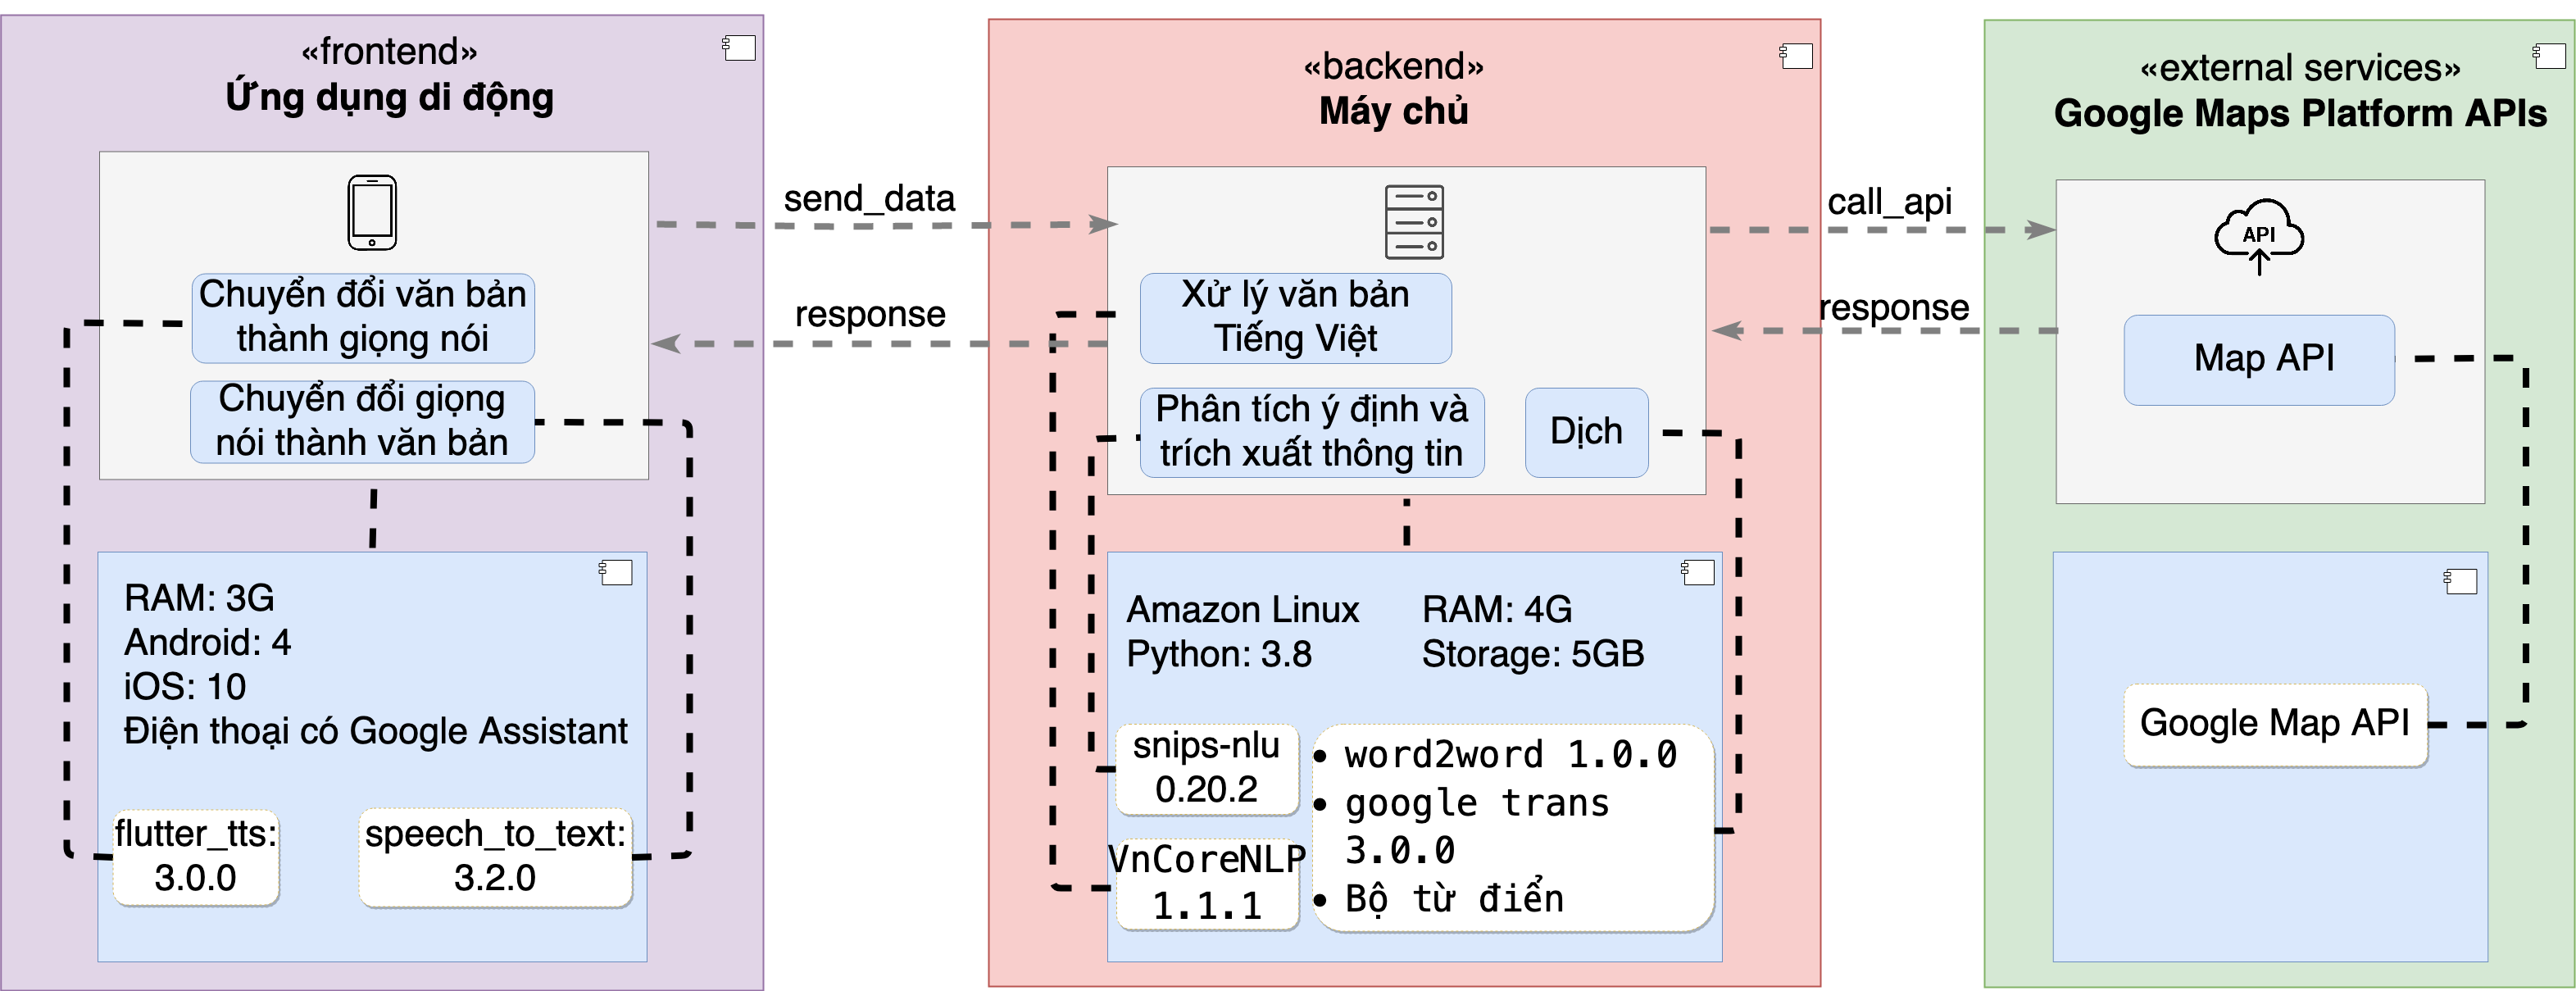
\includegraphics[width=10cm]{images/Structure-System.png}
    \caption{Kiến trúc hệ thống}
    \label{fig:kien-truc-he-thong}
\end{figure}

Máy chủ (Server) là chương trình xử lý và phân tích dữ liệu. Chương trình này chịu trách nhiệm xử lý dữ liệu gửi lên (Text) bao gồm hai thành phần: Phân tích ý định, trích xuất dữ liệu và tìm kiếm kết quả trả lời câu hỏi của người gửi. Khi ứng dụng điện thoại gửi Text lên, chương trình xử lý rồi trả về kết quả trên ứng dụng điện thoại. Máy chủ sẽ cung cấp các API tương ứng. Các API này sẽ có nhiệm vụ giao tiếp với chương trình xử lý ở máy chủ.

Trong phạm vi đề tài, nhóm sẽ xây dựng thành phần xác định ý định, trích xuất dữ liệu và tìm kiếm kết quả trả lời câu hỏi sẽ sử dụng API của Google Map\cite{google-map}. 

Phầm mềm ứng dụng cung cấp một giao diện người dùng qua ứng dụng trên điện thoại di động. Giao diện này cho phép người dùng sử dụng để hỏi các câu hỏi về chỉ đường từ một địa chỉ này đến một địa chỉ khác cụ thể bằng giọng nói (ghi âm câu nói) hoặc là nhập văn bản trên ứng dụng và trả về cho người dùng kết quả phù hợp.
\begin{itemize}
    \item[--] Chuyển giọng nói thành văn bản: Chuyển câu lệnh bằng giọng nói của người dùng thành văn bản để hiển thị lên ứng dụng và gửi lên hệ thống.
    \item[--] Chuyển văn bản thành giọng nói: Chuyển phản hồi của hệ thống thành dạng âm thanh để phát ra qua điện thoại.
\end{itemize}

\section{Xây dựng thành phần xác định ý định và trích xuất thực thể}
\subsection{Tạo dữ liệu tiếng Việt}
Nhóm đã thực hiện tạo dữ liệu gồm hai intent là findRoute và askLocation. Mỗi intent gồm 20 câu huấn luyện và 10 câu để kiểm thử.
\begin{itemize}
    \item[--] Tạo dữ liệu trên file txt. Với intent "findRouteAB" ta có câu ví dụ: "Đường đi từ đại học Sài gòn đến Cao đẳng sài gòn"
    \item[--] Chuyển dữ liệu sang dạng json để thuận tiện cho việc huấn luyện (Xem hình dữ liệu dưới dạng file json \ref{fig:data-train-json} ).
\end{itemize}
\begin{figure}[htp]
    \centering
    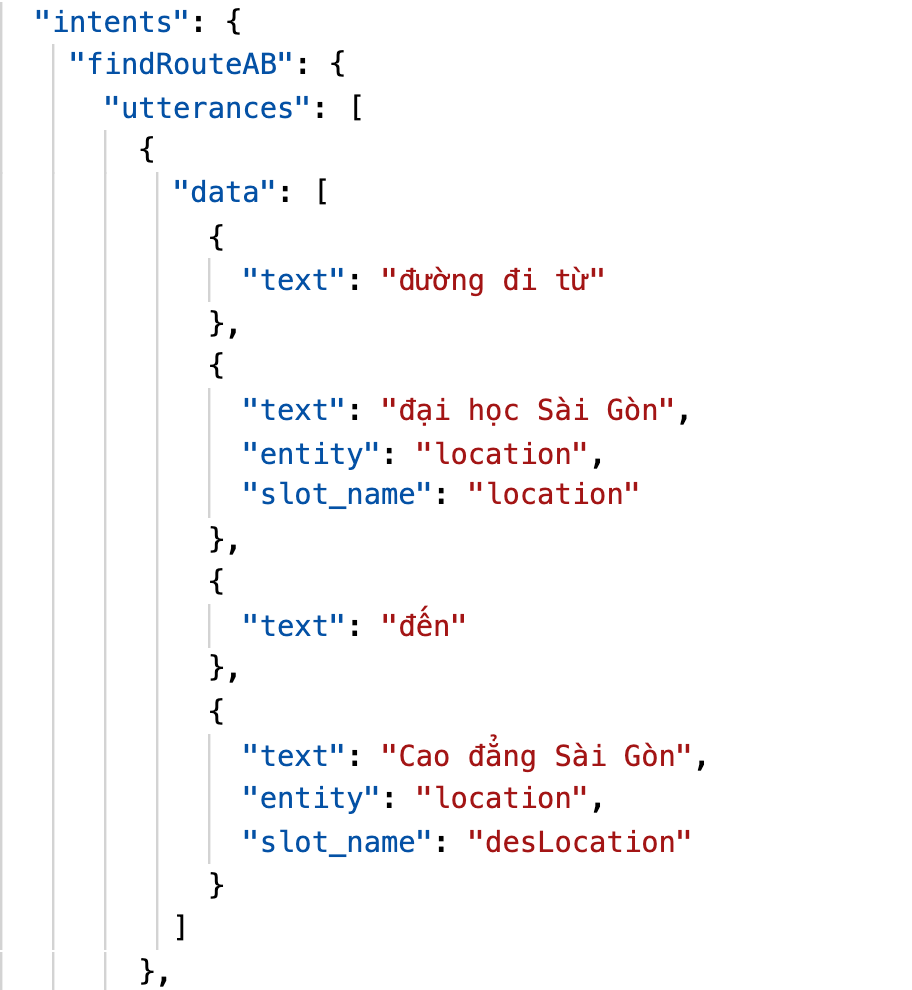
\includegraphics[width=10cm]{images/Data-train-json.png}
    \caption{Hình ảnh minh họa dữ liệu trước khi dịch và sau khi dịch}
    \label{fig:data-train-json}
\end{figure}

\subsection{Tiền xử lý dữ liệu, huấn luyện và kết quả}

Với dữ liệu được chuẩn bị để huấn luyện là tiếng Việt, nhưng dữ liệu để đưa vào mô hình huấn luyện là tiếng Anh, chúng em đã tiến hành chuyển hoá dữ liệu từ tiếng Việt sang tiếng Anh với các phương pháp khác nhau và thu được kết quả dưới đây.

\begin{enumerate}
    \item Word2word
          
          Đầu tiên, chúng em dịch bộ dữ liệu từng từ bằng cách tách 1 câu thành từng từ rồi sử dụng thư viện (word2word) để dịch sang tiếng Anh.Vd để dịch câu: "cách đi từ đại học Kinh Tế đến đại học Văn Lang".
          \begin{itemize}
              \item[--] Tách câu thành từng từ riêng biệt: ['cách', 'đi', 'từ', 'đại', 'học', 'Kinh' ,'Tế' ,'đến', 'đại', 'học', 'Văn', 'Lang']
              \item[--] Dịch từng từ sang tiếng Anh, ta được: ['ways', 'gone', 'word', 'Swordsman', 'learn', 'GrosDs', 'Monk', 'until', 'Swordsman', 'learn', 'Lam', 'Lang']
          \end{itemize}
          
          Sau khi dịch ta được bộ dữ liệu huấn luyện\footnote{Xem thêm về bộ huấn luyện \url{https://drive.google.com/file/d/1yoQk3AuViJpkcDQumQI-SbIw_iGyaGoJ/view?usp=sharing}} và bộ dữ liệu kiểm thử\footnote{Xem thêm về bộ kiểm thử \url{https://drive.google.com/file/d/1i2YNlvZTVsTU2WrzIMBmxl4FcJuAtVyV/view?usp=sharing}}
          \begin{figure}[htp]
              \centering
              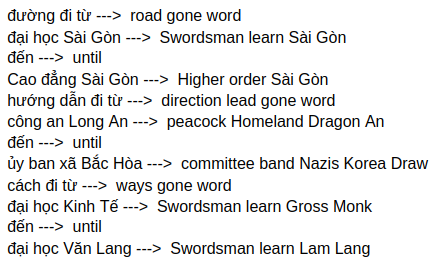
\includegraphics[width=10cm]{images/trainingdata_dichtungtu.png}
              \caption{Hình ảnh minh họa dữ liệu trước khi dịch và sau khi dịch}
              \label{fig:sodohethongchiduong}
          \end{figure}
          
          Đem bộ dữ liệu để huấn luyện và đánh giá, ta đạt được kết quả như hình 3.3, xem chi tiết \footnote{\url{https://drive.google.com/file/d/1e2Z0g4irQXqeNMzz4rP1UPQ3OKqYsMPI/view?usp=sharing}}:
          
          \begin{figure}[htp]
              \centering
              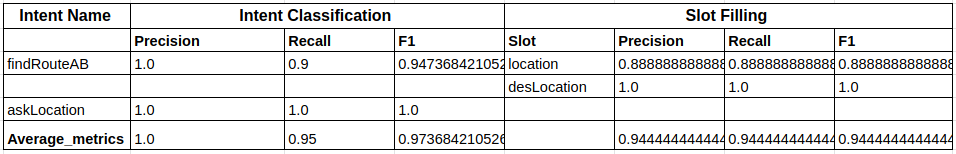
\includegraphics[width=15cm]{images/metrics-dich-tung-t.png}
              \caption{Các chỉ số của mô hình}
              \label{fig:sodohethongchiduong}
          \end{figure}
          Nhận xét kết quả đạt được:
          \begin{itemize}
              \item[--] Mặc dù kết quả tương đối tốt nhưng phương pháp dịch từng từ này không khả thi bởi vì sẽ mà mất ý nghĩa của câu nói, ví dụ như câu sau: "từ Đại học Khoa học Tự nhiên đến Đại học Bách khoa đi như thế nào" được dịch thành "word Swordsman learn department learn itself course until Swordsman learn centurion department" Các thực thể địa điểm như "Đại học Khoa học Tự nhiên" được dịch thành "Swordsman learn department learn itself course", "Đại học Bách khoa" dịch thành "Swordsman learn centurion department"
              \item[--] Các thực thể cần được trích xuất đã bị dịch ra và không còn ý nghĩa nữa, không thể dùng để tìm kiếm địa điểm này trên Google map được.
          \end{itemize}
    \item Áp dụng word segmentation và pos tagging lên bộ dữ liệu và sử dụng thư viện word2word
          
          Nhận thấy được vấn đề về các từ ghép và tên riêng sau khi dịch bằng phương pháp word2word không được chính xác và đúng ý nghĩa của câu. Chúng em tiến hành xem xét về vấn đề phân tách các từ. 
          
          Tách từ là một quát trình xử lý nhằm mục đích xác định ranh giới của các từ trong câu văn, cũng có thể hiểu đơn giản hơn là tách từ là quá trình xác định các từ đơn, từ ghép, danh từ,... có trong câu.
          
          Để xử lý vấn đề dịch các tên riêng và không đúng ngữ nghĩa, nhóm em thay đổi phương pháp dịch bằng cách sử dụng thư viện để tách từ (word segmentation) và gán nhãn từ loại (pos tagging).
          
          Trong tiếng Việt, dấu cách (space) không được sử dụng như 1 kí hiệu phân tách từ, nó chỉ có ý nghĩa phân tách các âm tiết với nhau. Do đó việc tách từ sẽ giúp cho việc dịch được chính xác hơn.
          
          Về vấn đề những slot bị dịch thành tiếng Anh làm cho nó không còn ý nghĩa nữa, nhóm em nhận thấy rằng những slot này chủ yếu là danh từ, nên nhóm sẽ sử dụng pos tagging để gán nhãn từ loại, những từ nào thuộc danh từ thì sẽ không cho dịch thành tiếng Anh.
          
          Áp dụng word segmentation và pos tagging lên bộ dữ liệu và sử dụng thư viện word2word để dịch thì đạt được bộ dữ liệu huấn luyện\footnote{\url{https://drive.google.com/file/d/1riZLV1dam9U6q5fuutBFZkzpC6IGgvbb/view?usp=sharing}} và bộ dữ iệu kiểm thử\footnote{	\url{https://drive.google.com/file/d/1Jq1x3-owrcL1TN1igPr7HFNRxTk2emW2/view?usp=sharing}}:
          
          \begin{figure}[htp]
              \centering
              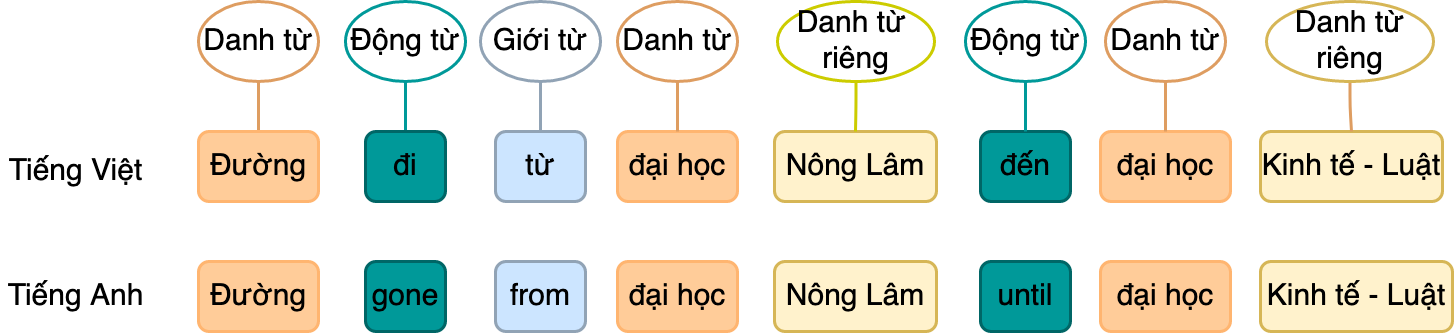
\includegraphics[width=10cm]{images/trainingdata-wordsegment.png}
              \caption{Hình ảnh minh họa dữ liệu trước khi dịch và sau khi dịch bằng phương pháp dùng word segmentation và pos tagging}
              \label{fig:sodohethongchiduong}
          \end{figure}
          
          Sau khi huấn luyện mô hình và đem đi đánh giá nhóm nhận được kết quả như  hình 3.4, xem chi tiết \footnote{\url{https://drive.google.com/file/d/1UU7_04Ps6WHZXSujZxNqaZKZhtvYsnrL/view?usp=sharing}}:
          
          \begin{figure}[htp]
              \centering
              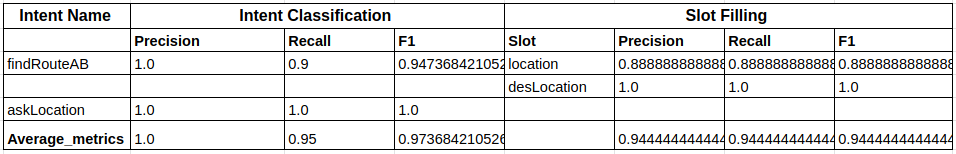
\includegraphics[width=15cm]{images/metrics-dich-tung-t.png}
              \caption{Các chỉ số của mô hình}
              \label{fig:sodohethongchiduong}
              
          \end{figure}
          
          Nhận xét kết quả đạt được:
          \begin{itemize}
              \item[--] Sau khi áp dụng tách từ và phân loại từ vựng, nhóm đã xử lý tương đối được vấn đề dịch những slot làm mất ý nghĩa của chúng: "từ Đại học Khoa học Tự nhiên đến Đại học Bách khoa đi như thế nào" được dịch thành "word đại\_học khoa\_học\_tự\_nhiên until đại\_học bách\_khoa gone như\_thế\_nào"
          \end{itemize}
          Tuy nhiên vẫn còn một vài trường hợp dịch còn chưa ổn, ví dụ như "Đại học Khoa học Xã hội và Nhân văn" được dịch thành "Đại học Khoa học Xã hội their Nhân văn"
    \item Xây dựng bộ từ điển
          Để có thể xử lý tốt hơn về vấn đề ý nghĩa trong câu được dịch sang một cách chính xác hơn. Nhóm chúng em đã quyết định xây dựng mô hình so khớp dài nhất (longest matching), bằng cách xây dựng một bộ từ điển, và tìm từ dài nhất có trong bộ từ điển đó để tiến hành dịch. Bộ từ điển này nằm trong phạm vi hỏi đường nên có thể xây dựng với các từ ngữ cụ thể có trong chủ đề, từ đó việc dịch sẽ đạt hiệu quả hơn.
          
          Trong phạm vi các câu hỏi về đường đi, chúng em đã lựa chọn dịch khoảng 50 từ và các cụm từ. Các bước để dịch được dữ liệu như sau:
          \begin{itemize}
              \item[--] Bước 1: Xây dựng bộ từ điển riêng biệt về chủ đề hỏi đường đi và chuyển hoá từ ngôn ngữ tiếng Việt sang tiếng Anh.
              \item[--] Bước 2: Tìm từ dài nhất trong câu có trong bộ từ điển.
              \item[--] Bước 3: Lấy nghĩa của từ tương ứng trong từ điển.
          \end{itemize}
          Trong quá trình nghiên cứu, chúng em nhận thấy bước 2 là bước thật sự cần thiết để có thể tìm được từ thích hợp nhất với bộ từ điển để có kết quả tốt nhất. Dưới đây là mô tả quá trình tìm từ dài nhất có trong từ điển mà nhóm chúng em thực hiện (Xem hình Tìm từ dài nhất \ref{fig:longest-word})
          \begin{itemize}
              \item[--] Input: "Đường đi từ Đại học Nông Lâm đến Ngã tư Thủ Đức""
              \item[--] Output: ["Đường đi", "từ", "Đại học Nông Lâm", "đến", "Ngã tư Thủ Đức"]
          \end{itemize}
          \begin{figure}[htp]
              \centering
              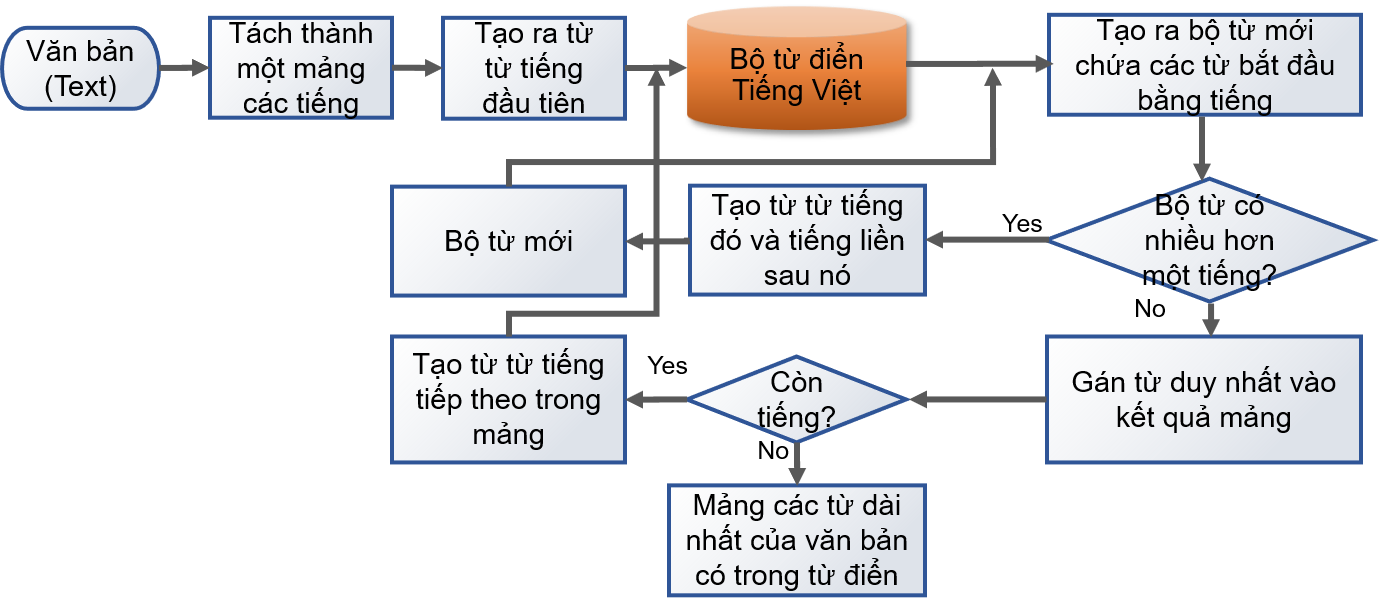
\includegraphics[width=10cm]{images/Diagram-longest-word.png}
              \caption{Tìm từ dài nhất}
              \label{fig:longest-word}
          \end{figure}
          
          Sau khi dịch ta được bộ dữ liệu huấn luyện\footnote{\url{https://drive.google.com/file/d/1l6TW8QdhZYOC7uhCpIJpsuSwVfrSv5ie/view?usp=sharing}} và bộ dữ liệu kiểm thử \footnote{\url{https://drive.google.com/file/d/1DpIxFSOjwP_djW-V1jpaLH4HTwGgGZkA/view?usp=sharing}}
          \begin{figure}[htp]
              \centering
              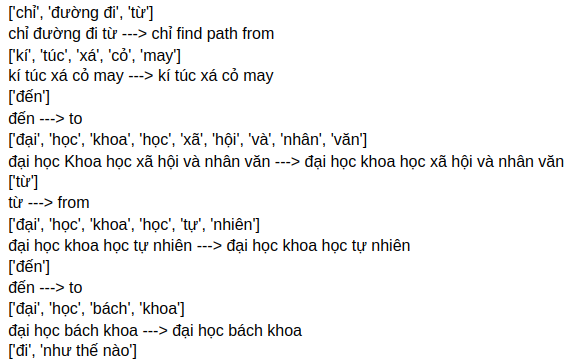
\includegraphics[width=10cm]{images/trainingdata-tudien.png}
              \caption{Hình ảnh minh họa dữ liệu trước khi dịch và sau khi dịch bằng phương pháp xây dựng từ điển}
              \label{fig:sodohethongchiduong}
              
          \end{figure}
          
          Đem bộ dữ liệu để huấn luyện và đánh giá, ta đạt được kết quả như hình 3.8, xem chi tiết \footnote{\url{https://drive.google.com/file/d/1HSe-ri76d8jbF3FZUCrDiFawHI17D18a/view?usp=sharing}}:
          
          \begin{figure}[htp]
              \centering
              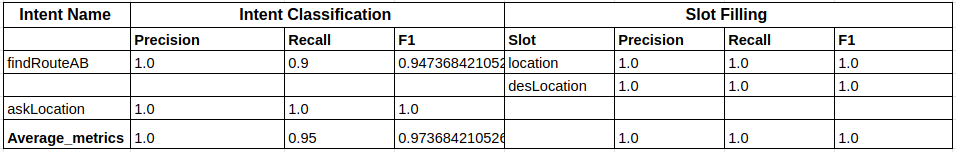
\includegraphics[width=15cm]{images/metrics-tudien.png}
              \caption{Các chỉ số của mô hình}
              \label{fig:sodohethongchiduong}
          \end{figure}
          Kết quả đạt được sau khi dùng phương pháp dịch bằng cách xây dựng bộ từ điển:
          \begin{itemize}
              \item[--] Do xây dựng bộ từ điển những từ vựng trong phạm vi nhỏ - hỏi đường nên bộ dịch cho ra kết quả khá khả quan, cải thiện hơn so với 2 phương pháp trước là phương pháp dịch từng từ và phương pháp dịch dùng word segmentation và pos tagging
              \item[--] Kế hoạch phát triển là xây dựng thêm dữ liệu, tạo thêm nhiều ý định sau đó thực hiện đánh giá mô hình để xem mô hình có thực sự hiệu quả hay không.
          \end{itemize}
\end{enumerate}